\chapter{Documentation}

During the study thesis documentation for the OSM2VectorTiles project was created. It was decided to separate the documentation into a user-centric and a developer-centric part. All of this information was provided on the project website (\url{http://osm2vectortiles.org}). When the project was publicly released and people started to get interested in this project, two main problems with the documentation were discovered:

\begin{itemize}
    \item The tutorials targeted to regular users were too complicated and error prone
    \item Developers want to have the documentation in the Github repository right next to the code not on the project website
\end{itemize}

With this knowledge it was decided to move the developer-centric documentation into readme files right next to the code and simplify the user-centric tutorials to eliminate most beginner errors.

\begin{figure}[H]
  \centering
  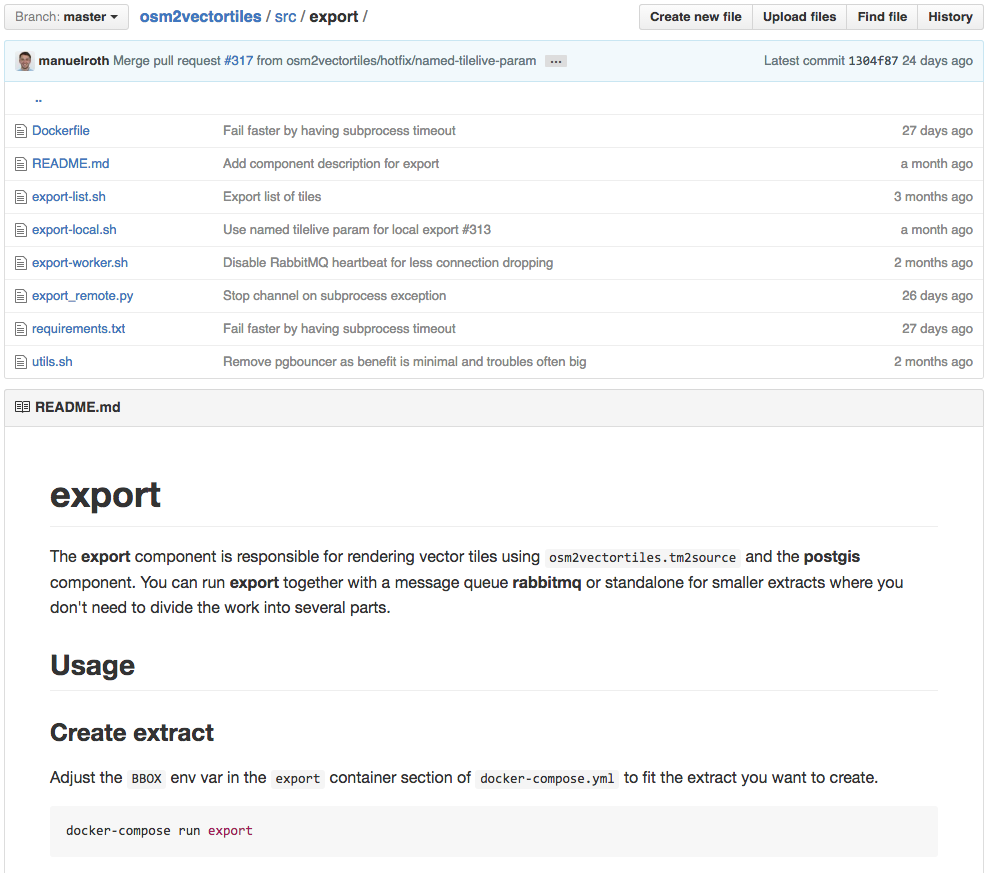
\includegraphics[width=1.0\textwidth]{images/documentation/developer_documentation}
  \caption{Documentation of the export component using a readme file}
  \label{developer_documentation}
\end{figure}

\autoref{developer_documentation} and \autoref{user_documentation} show the documentation in the repository on Github and on the project website. The documentation isn't part of this thesis therefore can be found either on Github or the project website.

\begin{figure}[H]
  \centering
  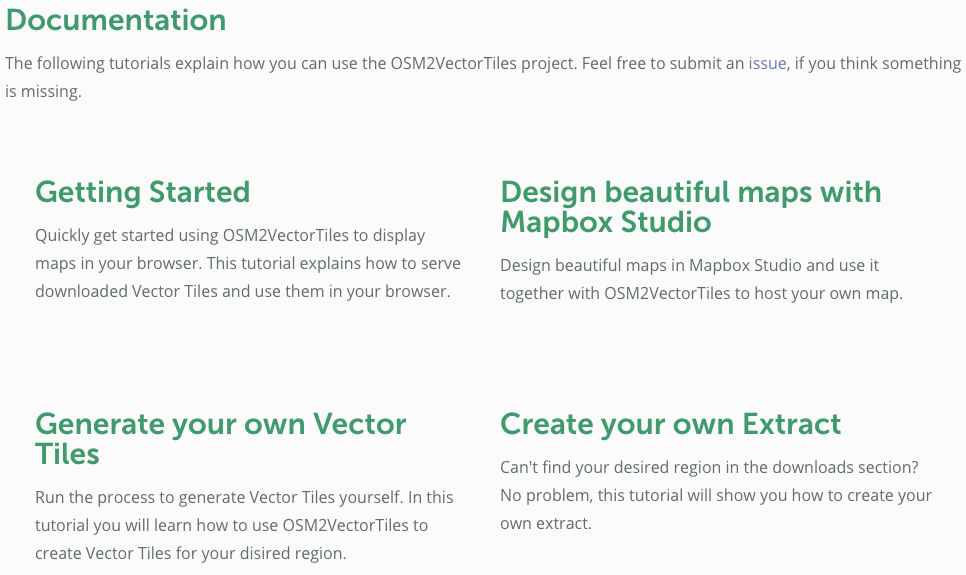
\includegraphics[width=1.0\textwidth]{images/documentation/user_documentation}
  \caption{Simplified overview of user documentation on the project website}
  \label{user_documentation}
\end{figure}